\subsection{Problems with assignment ``=''}
\begin{itemize}
	\item Same issue with copy constructor, it does a shallow copy
	\item \textbf{Operator overloading} lets us customize what happens when we use a built-in symbol.
\begin{lstlisting}[style=C++]
class IntSet{
	// data elements
	// ...

public:
	// Constructors
	// EFFECTS: assignment operator does a deep copy
	IntSet &operator= (const IntSet &rhs);
	//...
};
\end{lstlisting}
	\item Like the copy constructor, the assignment operator takes a reference to a const instance to copy from
	\item However, it also returnsa reference to the copied-to object.
	\item This return value allows for a chained assignmentlike this: \lstinline[style=C++]{is3 = is2 = is1; }
\end{itemize}

\subsection{Understanding this}
\begin{itemize}
	\item We need to return a reference to the current \lstinline[style=C++]{IntSet} so that chaining works
	\item Every member function has a ``secret'' variable called \lstinline[style=C++]{this}
	\begin{itemize}
		\item \lstinline[style=C++]{this} is a pointer to the current instance of the class
		\item Here, we use \lstinline[style=C++]{*this} because the reutrn type isa reference
	\end{itemize}
	\item Think of \lstinline[style=C++]{this} as a local variable which points to the current instance
	\begin{center}
		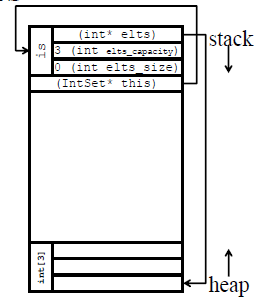
\includegraphics{sections/lec17/this.png}
	\end{center}
\end{itemize}

\subsection{The Rule of the Big Three}
\begin{itemize}
	\item If you have any dynamically allocated storage in a class, you must provide:
	\begin{enumerate}
		\item A destructor
		\item A copy constructor
		\item An overloaded assignment operator
	\end{enumerate}
\end{itemize}